\section{Introduzione}
\label{section:introduzione}

Il capitolo corrente fa da introduzione al lavoro svolto e orienta il lettore 
ad alcuni aspetti principali che interessano il campo del ``Spreading Rumors''.

I primi studi riguardanti la diffusione di una notizia risalgono ai primi anni '60~\cite{biblio:stochastic_rumours}, 
ma quelli presi in considerazione in questo lavoro sono più attuali e riguardano il campo dei Social Networks.

Lo studio della propagazione di una ``voce'', definita più semplicemente notizia o informazione, 
serve ad analizzare alcuni comportamenti, paramenti e modelli di una rete sociale.
Le caratteristiche principali sono la topologia della rete e gli utenti che ne fanno parte.

Possiamo quindi iniziare a dire che le simulazioni prevederanno una rete di utenti che ``a contatto'' con
la notizia decideranno a loro volta se ricondividerla o solamente prendere atto della sua esistenza.
Al passo 0 della simulazione verrà scelto un utente a cui verrà ``insegnata'' l'informazione 
che dovrà essere propagata. 
Facendo un riferimento al tema della medicina, durante un'indagine epidemiologica, il primo paziente ad aver 
contratto la malattia viene chiamato paziente zero.
Nel nostro caso non si tratta di una malattia ma di una notizia.

Durante le simulazioni verranno inoltre utilizzati alcuni termini che definirò qua di seguito:
\begin{itemize}
 \item ``Ignorants''\cite{biblio:spread_rumor} : al momento della creazione della rete sociale tutti gli utenti vengono definiti 
 in tal modo perchè non sono al corrente della notizia;
 \item ``Spreaders''\cite{biblio:spread_rumor} : tutti gli utenti che decidono di condividere la notizia. 
 Il ``paziente zero'' fa parte di questo gruppo;
 \item ``Uninterested'' : tutti quegli utenti che dopo essere diventati consapevoli dell'esistenza 
 della notizia decidono comunque di non condividerla;
 \item ``Viewers'' o visualizzatori : tutti coloro facenti parte del gruppo degli Spreaders e degli Uninterested.
\end{itemize}

Facendo una veloce panoramica, l'argomento di questo progetto è certamente un ottimo ambiente di studio
ed il numero esorbitante di utilizzatori di Social Networks in circolazione crea sicuramente 
un terreno fertile per la diffusione di notizie ed informazione.




\subsection{Obiettivi}
\label{section:obiettivi}

Per questo lavoro possiamo definire tre obiettivi principali.

Il primo test permetterà di decidere il modello topologico più consono, tra quelli 
presi in considerazione, per i successivi test.

Il secondo servirà per mettere in luce come una notizia, 
con un topic adatto maggiormente ad una certa fascia d'età, venga diffusa nei differenti Social Networks.
E' presente una statistica online piuttosto recente (3\degree trimestre 2014) che mostra la distribuzione 
per età di come è divisa l'utenza nei social networks più popolari. 
Il grafico in figura~\ref{img:age_distribution_social} ne mostra la distribuzione.

\begin{figure}[!ht]
 \centerline{
  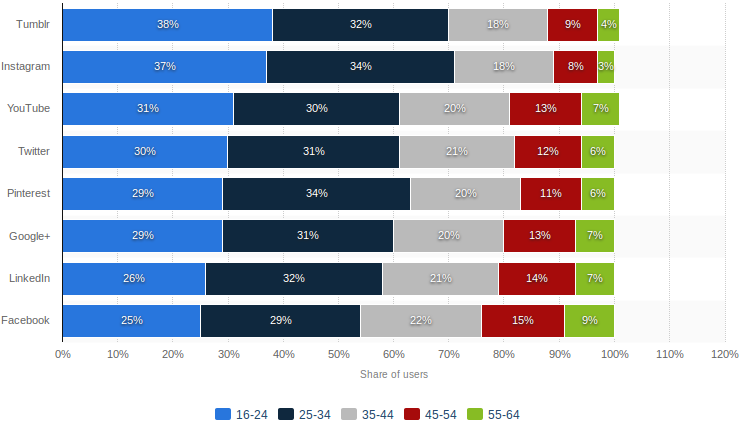
\includegraphics[width=0.8\textwidth]{img/age-distribution.png}
 }
\caption{Distribuzione delle età divisa per Social Network ~\cite{biblio:age_distribution_social}}
\label{img:age_distribution_social}
\end{figure}


L'ultimo obiettivo, invece, servirà ad analizzare un'interazione tra 2 diversi gruppi di utenti, che 
permetterà di studiare il numero di visualizzazioni della notizia in casi più complessi.
Un esempio potrebbe essere quello di voler dividere il numero totale delle persone in due sottoinsiemi così formati:
\begin{itemize}
 \item Il primo gruppo è formato da pochi utenti, tipo il 20\% del totale, ma ogni componente ha un'ottima probabilità di condivisione.
 \item Il secondo gruppo, viceversa, è formato dall'80\% degli utenti, ma ogni componente ha una possibilità minore di condivisione.
\end{itemize}





